\documentclass[border=10pt]{standalone}
\usepackage[utf8]{inputenc}
\usepackage[T1]{fontenc}
\usepackage{tikz}
\usetikzlibrary{shapes.geometric, arrows.meta, positioning, fit, backgrounds, shadows}

\begin{document}

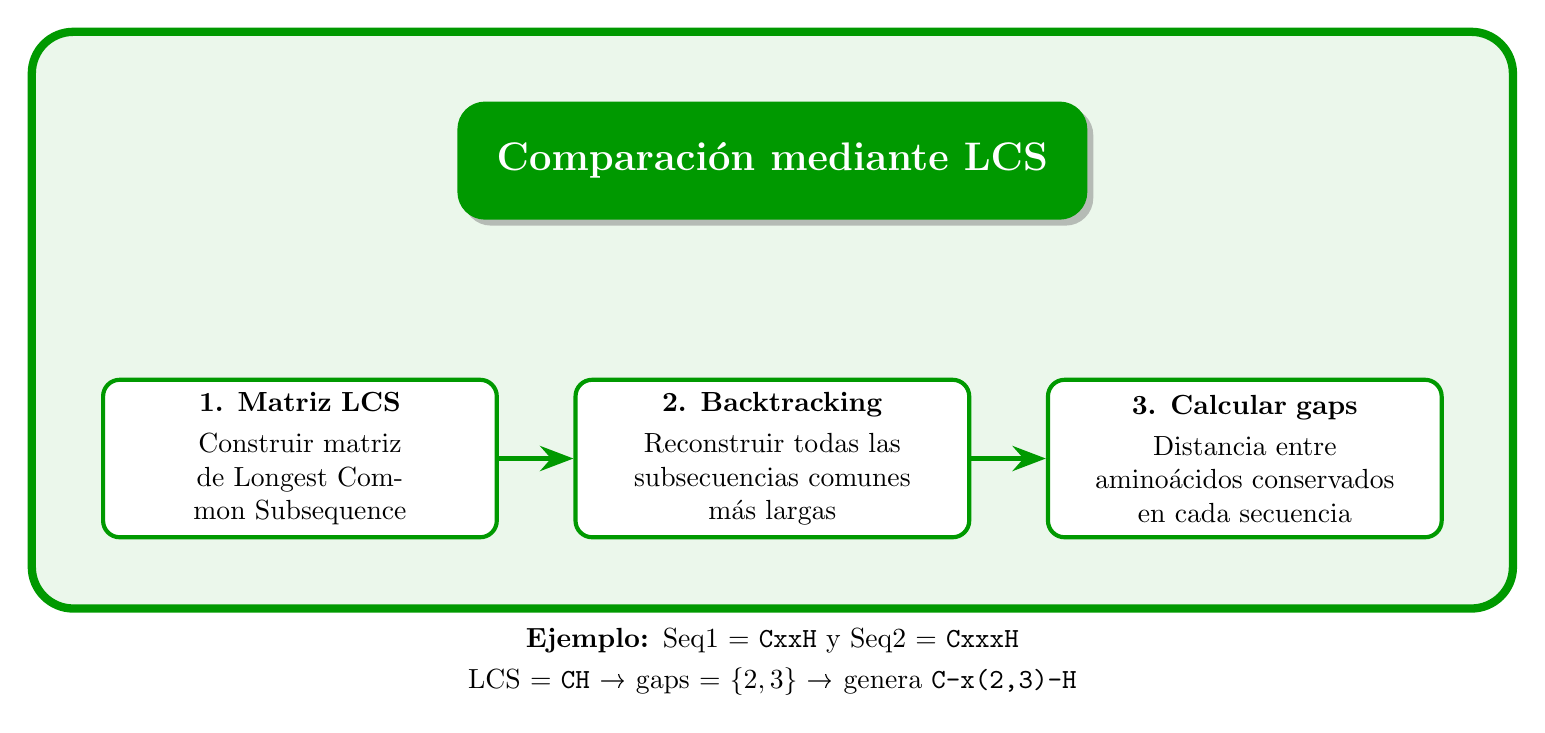
\begin{tikzpicture}[
        node distance=1.5cm,
        % Estilos para nodos principales
        mainbox/.style={
                rectangle,
                rounded corners=10pt,
                minimum width=8cm,
                minimum height=1.5cm,
                text centered,
                text width=7.5cm,
                font=\bfseries\Large,
                text=white,
                drop shadow
            },
        % Estilos para sub-nodos
        subbox/.style={
                rectangle,
                rounded corners=6pt,
                minimum width=5cm,
                minimum height=2cm,
                text centered,
                text width=4.5cm,
                font=\normalsize,
                text=black,
                fill=white,
                draw=green!60!black,
                line width=1.5pt
            },
        % Flechas
        arrow/.style={
                ->,
                >=Stealth,
                line width=2pt,
                color=green!60!black
            },
        % Grupo contenedor
        groupbox/.style={
                rectangle,
                rounded corners=15pt,
                draw=green!60!black,
                line width=3pt,
                fill=green!60!black!8,
                inner sep=25pt
            }
    ]

    % Título principal
    \node[mainbox, fill=green!60!black] (comparacion) {Comparación mediante LCS};

    % Sub-nodos
    \node[subbox, below=2cm of comparacion, xshift=-6cm] (comp1) {
        \textbf{1. Matriz LCS}\\[3pt]
        Construir matriz\\
        de Longest Common Subsequence
    };

    \node[subbox, below=2cm of comparacion] (comp2) {
        \textbf{2. Backtracking}\\[3pt]
        Reconstruir todas las\\
        subsecuencias comunes\\
        más largas
    };

    \node[subbox, below=2cm of comparacion, xshift=6cm] (comp3) {
        \textbf{3. Calcular gaps}\\[3pt]
        Distancia entre\\
        aminoácidos conservados\\
        en cada secuencia
    };

    % Grupo
    \begin{scope}[on background layer]
        \node[groupbox, fit=(comparacion)(comp1)(comp2)(comp3)] (gcomp) {};
    \end{scope}

    % Flechas entre sub-nodos
    \draw[arrow] (comp1.east) -- (comp2.west);
    \draw[arrow] (comp2.east) -- (comp3.west);

    % Ejemplo
    \node[below=1cm of comp2, text width=14cm, align=center, font=\normalsize] (ejemplo) {
        \textbf{Ejemplo:} Seq1 = \texttt{CxxH} y Seq2 = \texttt{CxxxH}\\[3pt]
        LCS = \texttt{CH} → gaps = $\{2, 3\}$ → genera \texttt{C-x(2,3)-H}
    };

\end{tikzpicture}

\end{document}
